\documentclass{beamer}

\usepackage{amsmath, amssymb}
\usepackage{graphicx}
\usepackage{url}
\usepackage{xspace}
\usepackage{pifont}
\usepackage{minted}
\usepackage{verbatim}
\usepackage{wasysym}
\usepackage[numberedbib]{apacite}
\usepackage{bm}

\DeclareMathOperator{\Tr}{Tr}

\usetheme{AnnArbor}
\usefonttheme[onlymath]{serif}

\title[Intro DNNs]{\textbf{Practical Deep Neural Networks} \\
\textbf{\normalsize GPU computing perspective}\\
\normalsize Convolutional Neural Networks}
\author{Yuhuang Hu \and Chu Kiong Loo}
\institute[UM]{Advanced Robotic Lab\\
Department of Artificial Intelligence\\
Faculty of Computer Science \& IT\\
University of Malaya}

\date{}

\begin{document}

\frame{\titlepage}

\begin{frame}
  \frametitle{Outline}

  \tableofcontents
\end{frame}

\AtBeginSection[]
  {
     \begin{frame}
     \frametitle{Outline}
     \tableofcontents[currentsection]
     \end{frame}
  }

\section{Introduction}

\begin{frame}
  \frametitle{Assumed prerequisites}

  \begin{itemize}
    \item[\ding{80}] Basic signal processing
    \item[\ding{80}] MLP Network (DL book chapter 6)
  \end{itemize}

\end{frame}

\begin{frame}
  \frametitle{Suggest Readings}

  \begin{itemize}
    \item[\ding{45}] CS231n: \href{http://cs231n.github.io/convolutional-networks/}{Convolutional Neural Networks}, \href{http://cs231n.github.io/understanding-cnn/}{Visualize ConvNet}

    \item[\ding{45}] UFLDL Tutorial: \href{http://ufldl.stanford.edu/tutorial/supervised/FeatureExtractionUsingConvolution/}{Feature Extraction Using Convolution}, \href{http://ufldl.stanford.edu/tutorial/supervised/Pooling/}{Pooling}
    \item[\ding{45}] \href{http://www.iro.umontreal.ca/~bengioy/dlbook/convnets.html}{Deep Learning Book chapter 9}
    \item[\ding{45}] DL Tutorial: \href{http://deeplearning.net/tutorial/lenet.html}{Convolutional Neural Networks (LeNet)}
  \end{itemize}
\end{frame}

\section{Convolution}

\begin{frame}
  \frametitle{Convolution operation}

  \begin{equation*}
    s(t)=\int x(a)w(t-a)\, da
  \end{equation*}
  the operation is called \emph{convolution}. The convolution operation is typically denoted with $*$:
  \begin{equation*}
    s(t)=(x*w)(t)
  \end{equation*}
  In discrete form:
  \begin{equation*}
    s[t]=(x*w)(t)=\sum_{a=-\infty}^{\infty}x[a]w[t-a]
  \end{equation*}
\end{frame}

\begin{frame}
  \frametitle{2D convolution operation}

  \begin{equation*}
    s[i,j]=(I*K)[i,j]=\sum_{m}\sum_{n}I[m,n]K[i-m, j-n]
  \end{equation*}
  or equivalently:
  \begin{equation*}
    s[i,j]=(I*K)[i,j]=\sum_{m}\sum_{n}I[i-m, j-n]K[m,n]
  \end{equation*}
\end{frame}

\begin{frame}
  \frametitle{2D convolution operation}
  
 \begin{figure}
    \centering
    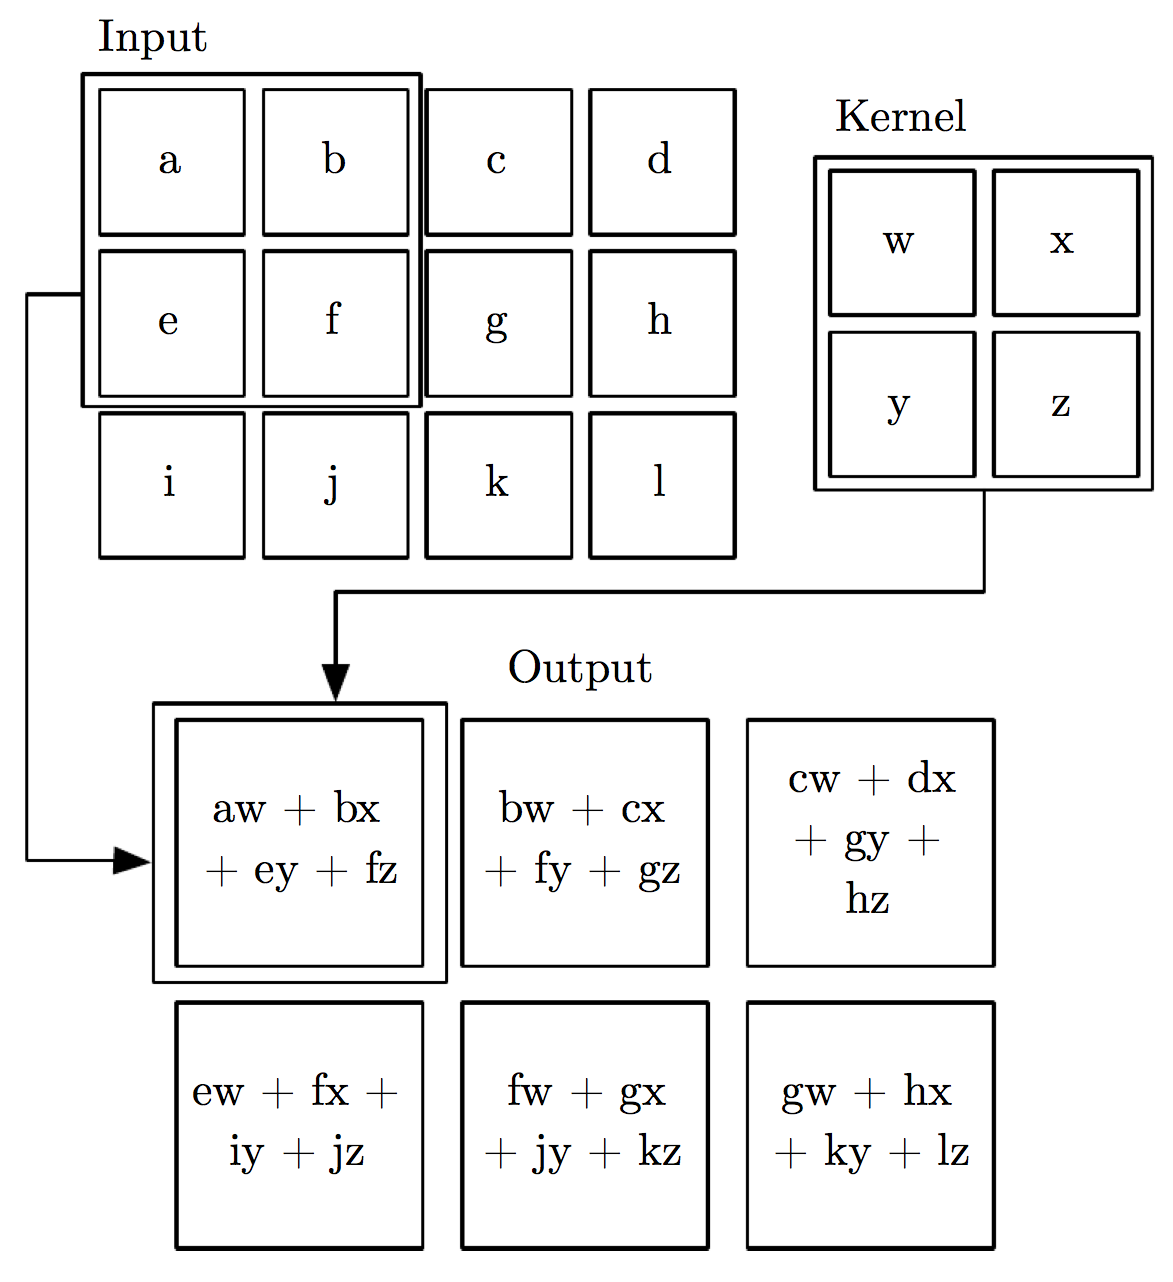
\includegraphics[width=0.55\textwidth]{convolution_operation.png}
  \end{figure}
\end{frame}

\section{Convolutional Neural Networks}

\begin{frame}
  \frametitle{LeNet-5}
  \begin{figure}[!htm]
    \centering
    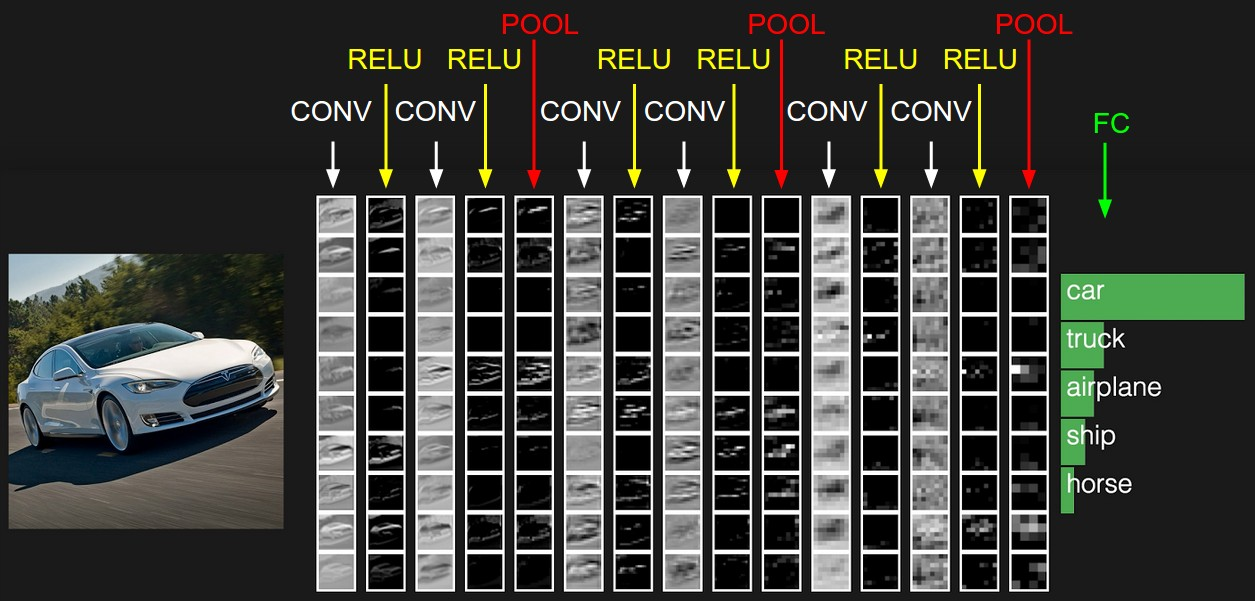
\includegraphics[width=0.8\textwidth]{convnet.jpeg}
  \end{figure}
\end{frame}

\begin{frame}
  \frametitle{MLP$\rightarrow$ConvNet}

  \begin{figure}[!htm]
    \centering
    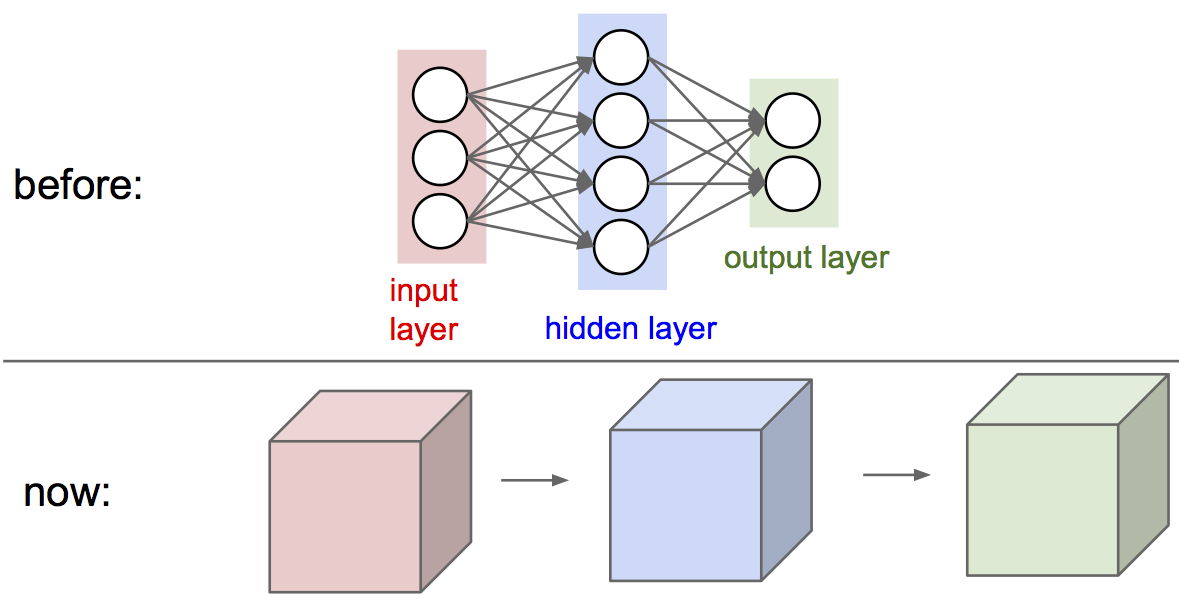
\includegraphics[width=0.8\textwidth]{convnet_gist.png}
  \end{figure}
\end{frame}

\begin{frame}
  \frametitle{Feature maps: activations of ConvNets}
  
  \begin{minipage}{0.48\textwidth}
    \begin{figure}[!htm]
      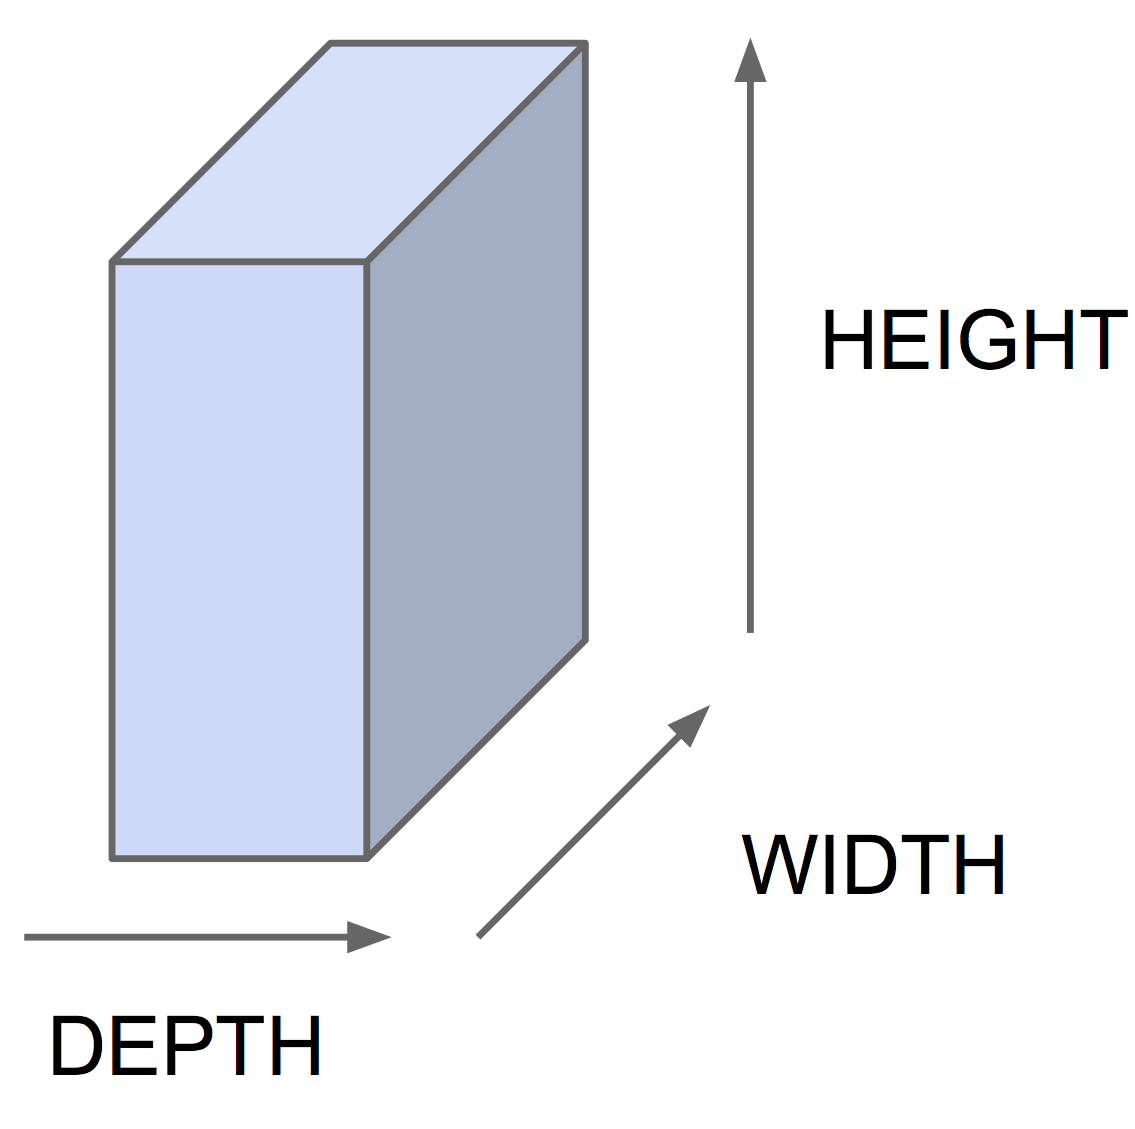
\includegraphics[width=0.8\textwidth]{feature_maps.png}
    \end{figure}
  \end{minipage}
  \begin{minipage}{0.48\textwidth}
    \begin{itemize}
      \item Network activations in ConvNets are \textbf{feature maps}.
      \item All ConvNets feature maps arranged in \textbf{3 dimensions}.
      \item Each feature maps has size of (HEIGHT, WIDTH)
      \item Input image can be a special kind of feature map (\emph{e.g.} color image is feature maps of some size with depth 3, one for each RGB channel).
    \end{itemize}
  \end{minipage}
\end{frame}

\begin{frame}
  \frametitle{Convolution Layer: simple cell}

  \begin{equation*}
    \mathbf{h}^{(k)}=f(\mathbf{x}*\mathbf{W}^{(k)}+b_{k})
  \end{equation*}

  \begin{itemize}
    \item Accepts a volume of size $W_{1}\times H_{1}\times D_{1}$
    \item Number of filters $K$ with shape $F\times F\times D_{1}$, stride $S$, amount of zero-padding $P$
    \item Produce a volume of size $W_{2}\times H_{2}\times D_{2}$ where
      \begin{align*}
        W_{2}&=(W_{1}-F+2P)/S+1 \\
        H_{2}&=(H_{1}-F+2P)/S+1 \\
        D_{2}&=K
      \end{align*}
  \end{itemize}

  \href{http://rt.dgyblog.com/res/dlworkshop/conv_demo.html}{Live Demo of convolution}
\end{frame}

\begin{frame}
  \frametitle{Pooling Layer: complex cell}

  \begin{figure}
    \centering
    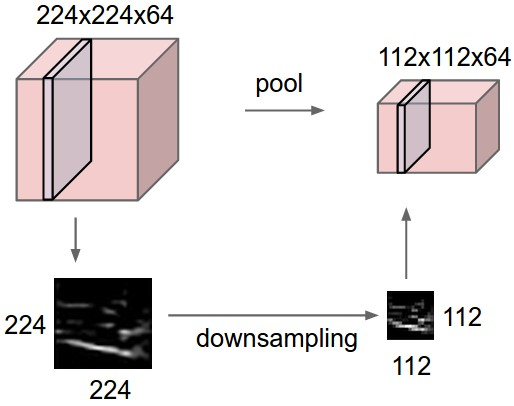
\includegraphics[width=0.25\textwidth]{pool.jpeg}\\
    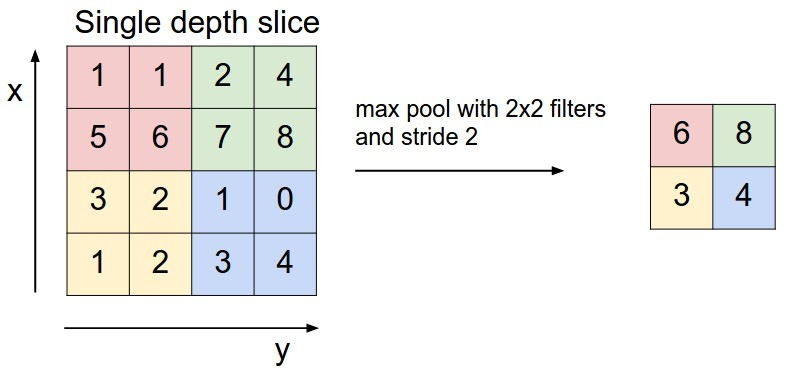
\includegraphics[width=0.5\textwidth]{maxpool.jpeg}
  \end{figure}
\end{frame}

\begin{frame}
  \frametitle{Live Demo}

  \begin{center}
    \emph{Running ConvNets on your browser!}
    \vspace{1cm}
    
    \href{http://cs.stanford.edu/people/karpathy/convnetjs/demo/cifar10.html}{Demo}\footnote{taken from Andrej Karpathy's ConvNetJS}
  \end{center}
  
\end{frame}

\section*{Q\&A}

\begin{frame}
  \frametitle{Q\&A}
  \begin{figure}
    \centering
    
\includegraphics[width=0.7\textwidth]{convnet_how_to_work.png}
  \end{figure}
\end{frame}

\end{document}
%%% Local Variables:
%%% mode: latex
%%% TeX-master: t
%%% End:
